\documentclass[12pt]{article}

\usepackage{amsmath}
\usepackage{amsfonts}
\usepackage{float}
\usepackage{fancyhdr}
\usepackage{graphicx}
\usepackage{placeins}
\usepackage[colorlinks=true,linkcolor=blue, citecolor=red]{hyperref}
\usepackage{url}
\usepackage[top=.75in, left=.75in, right=.75in, bottom=1in]{geometry}
\usepackage{arydshln}
\usepackage[utf8]{vietnam}
\setlength{\headheight}{29.43912pt}

\usepackage{mathptmx}
% \graphicspath{PATH_TO_GRAPHIC_FOLDER}

\pagestyle{fancy}
\fancyfoot{}
\fancyfoot[R]{Page \thepage}

\newcommand{\reporttitle}{Báo cáo Seminar}
\newcommand{\coursename}{Khai thác ngữ liệu văn bản nâng cao (MTH089)}
\newcommand{\reportname}{ViHealthBERT: Pre-trained Language Models for Vietnamese \\ in Health Text Mining}

\lhead{
\reporttitle
}
\rhead{
Trường Đại học Khoa học Tự nhiên - ĐHQG HCM\\
Khai thác ngữ liệu văn bản nâng cao (MTH089)
}
\lfoot{\LaTeX\ template by \href{https://github.com/trhgquan}{Quan, Tran Hoang}}

\begin{document}
\begin{titlepage}
\newcommand{\HRule}{\rule{\linewidth}{0.5mm}}
\centering

\textsc{\LARGE đại học quốc gia tphcm}\\[1.5cm]
\textsc{\Large trường đại học khoa học tự nhiên}\\[0.5cm]
\textsc{\large khoa công nghệ thông tin}\\[0.5cm]
% \textsc{bộ môn công nghệ tri thức}\\[0.5cm]

\HRule \\[0.4cm]
{ 
\huge{\bfseries{\reporttitle}}\\[0.5cm]
\large{\bfseries{Đề tài: \reportname}}
}\\[0.4cm]
\HRule \\[0.5cm]

\textbf{\large Môn học: \coursename}\\[0.5cm]

\begin{minipage}[t]{0.4\textwidth}
\begin{flushleft} \large
\emph{Học viên thực hiện:}\\
Trần Hoàng Quân (19120338) \\
Phạm Anh Việt \textsc{(20C11060)} \\
Nguyễn Đức Thuận \textsc{(21C11035)} \\
Nguyễn Thiện Dương \textsc{(21C12004)} \\
\end{flushleft}
\end{minipage}
~
\begin{minipage}[t]{0.4\textwidth}
\begin{flushright} \large
\emph{Giáo viên hướng dẫn:} \\
% Dr. James \textsc{Smith}
TS. Nguyễn Trường Sơn\\
TS. Nguyễn Tiến Huy
\end{flushright}
\end{minipage}\\[1cm]

{\large \today}\\[1cm]


\includegraphics[scale=.3]{img/hcmus-logo.png}\\[1cm] 

\vfill
\end{titlepage}
\tableofcontents
\pagebreak

\section{Tóm tắt nội dung}
Các mô hình ngôn ngữ (Language Models - LM) được xây dựng và ứng dụng rộng rãi trong lĩnh vực xử lý ngôn ngữ tự nhiên (NLP) đã đạt được nhiều kết quả đáng chú ý trong những năm gần đây. Đặc biệt, chất lượng các mô hình đơn ngữ được huấn luyện sẵn dành cho những ngôn ngữ bị hạn chế về tài nguyên ngữ liệu đã tăng đáng kể. Đối với Tiếng Việt, một số mô hình ngôn ngữ tổng quát (general-domain language models) như PhoBERT\cite{phobert} đã cho kết quả rất cao trên thực nghiệm. Mặc dù các mô hình ngôn ngữ tổng quát rất đa dạng nhưng có rất ít các mô hình ngôn ngữ đặc thù dành riêng cho một số lĩnh vực (specific-domain language models). Đã có nhiều bộ ngữ liệu Tiếng Việt dành riêng cho lĩnh vực y tế được công bố, tuy nhiên vẫn chưa có mô hình ngôn ngữ Tiếng Việt nào được phát triển và huấn luyện dành riêng cho các task liên quan tới y tế. Vì lí do đó, nhóm tác giả bài báo \textit{ViHealthBERT: Pre-trained Language Models for Vietnamese in Health Text Mining}\cite{minh-EtAl:2022:LREC} công bố bài báo với những đóng góp sau:
\begin{itemize}
\item Giới thiệu mô hình ViHealthBERT là mô hình ngôn ngữ Tiếng Việt đặc thù cho lĩnh vực y tế, đạt được state-of-the-art (SOTA) trên các downstream tasks \textit{Nhận dạng thực thể có tên (Named-Entity Recognition - NER)}, \textit{Phân định từ viết tắt (Acronym Disambiguation)} và \textit{Tóm tắt câu hỏi y khoa (FAQ Summarization)}.
\item Giới thiệu các bộ ngữ liệu \textit{Acronym Disambiguation (AD)} và \textit{Freqently Asked Question (FAQ) Summarization} là các bộ ngữ liệu đặc thù cho lĩnh vực y tế.
\end{itemize}
\section{Kiến trúc mô hình ViHealthBERT}
\subsection{Transformer và BERT}
Mô hình Transformer ứng dụng cơ chế self-attention và multi-head attention được giới thiệu lần đầu trong paper Attention is All You Need\cite{DBLP:journals/corr/VaswaniSPUJGKP17}. 
\begin{figure}[H]
\centering
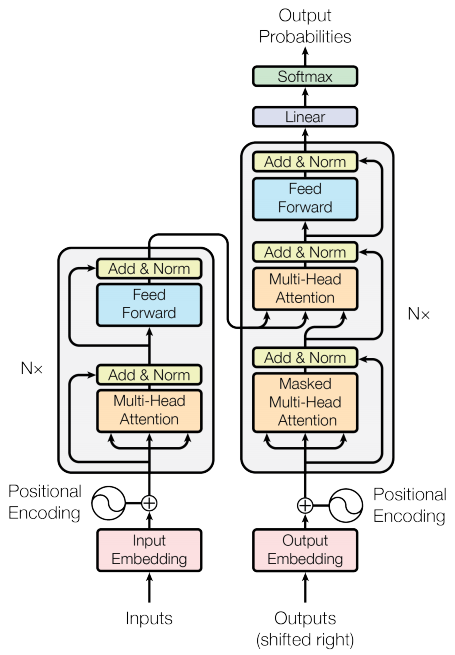
\includegraphics[scale=.35]{img/transformer.png}
\caption{Kiến trúc Transformer\cite{DBLP:journals/corr/VaswaniSPUJGKP17}}
\label{fig:transformer_diagram}
\end{figure}
Phần Encoder của Transformer được sử dụng trong mô hình BERT (\textbf{B}idirectional \textbf{E}ncoder \textbf{R}epresentations from \textbf{T}ransformers)\cite{devlin-etal-2019-bert}. Trong bài báo, BERT được giới thiệu có 2 phiên bản với các siêu tham số (hyperparameters) và số lượng tham số huấn luyện (training parameters) khác nhau:
\begin{itemize}
\item \textbf{BERT\textsubscript{base}}: 12 Transformer encoder layers, 768 hidden units, 12 attention heads, 110 triệu parameters.
\item \textbf{BERT\textsubscript{large}}: 24 Transformer encoder layers, 1024 hidden units, 16 attention heads và 340 triệu parameters.
\end{itemize}
\begin{figure}[H]
\centering
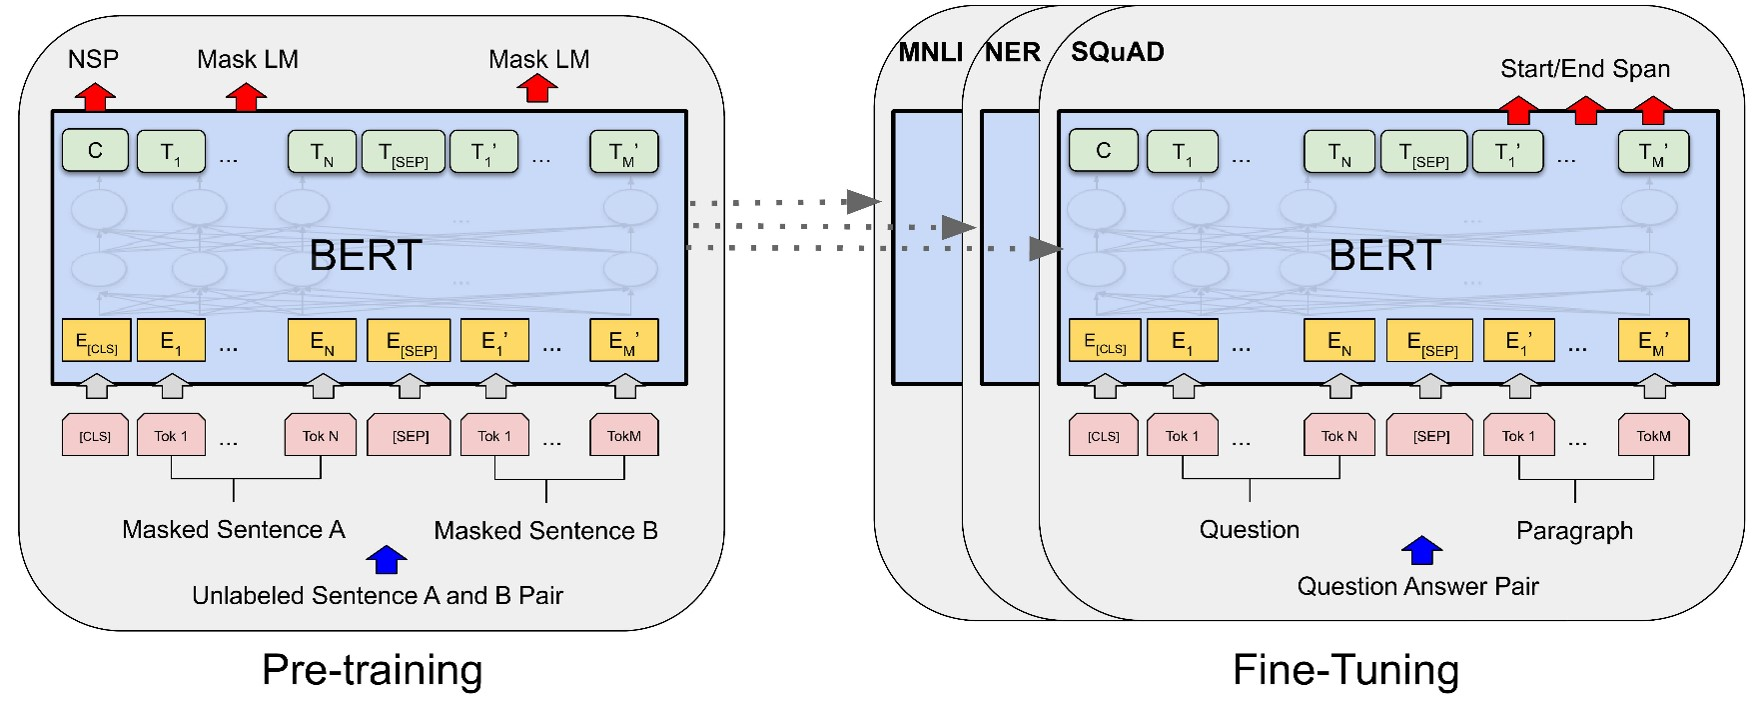
\includegraphics[scale=.65]{img/BERT.jpg}
\caption{Mô hình BERT\cite{devlin-etal-2019-bert}}
\label{fig:my_label}
\end{figure}
BERT được tiền huấn luyện (pretraining) với bộ ngữ liệu \textit{BookCorpus} (800 triệu từ) và \textit{Wikipedia English} (2500 triệu từ) với các pretraining task Masked Language Modeling (MLM) và Next Sentence Prediction (NSP), sau đó tinh chỉnh (finetune) lại cho từng task khác nhau. Sau khi BERT được công bố, nhiều mô hình cải tiến của BERT cũng được giới thiệu dựa trên kiến trúc của BERT, trong đó có thể kể đến
\begin{itemize}
\item \textbf{RoBERTa} (\textbf{R}obustly \textbf{o}ptimized \textbf{BERT} Pretraining \textbf{a}pproach)\cite{DBLP:journals/corr/abs-1907-11692}: sử dụng dynamic masking so với sử dụng static masking trong kiến trúc gốc; huấn luyện trên nhiều ngữ liệu hơn.
\item \textbf{DistilBERT}\cite{DBLP:journals/corr/abs-1910-01108}: mô hình nhỏ, nhanh, tốn ít chi phí huấn luyện hơn mô hình BERT gốc: có ít hơn 40\% parameters, chạy nhanh hơn 60\% nhưng hiệu quả bằng 95\% so với mô hình gốc.
\end{itemize}

\subsection{PhoBERT}
Dựa trên mô hình BERT, nhóm nghiên cứu từ VinAI đã công bố PhoBERT\cite{phobert}, được giới thiệu là mô hình ngôn ngữ đơn ngữ dành cho tiếng Việt có quy mô lớn đầu tiên. PhoBERT sử dụng quá trình pretraining của RoBERTa để tăng hiệu quả cho mô hình. Kiến trúc của PhoBERT vẫn giữ nguyên so với BERT:
\begin{itemize}
\item \textbf{PhoBERT\textsubscript{base}}: 12 encoder layers, 768 hidden units, 12 attention heads, 135 triệu parameters.
\item \textbf{PhoBERT\textsubscript{large}}: 24 encoder layers, 1024 hidden units, 16 attention heads và 370 triệu parameters.
\end{itemize}
PhoBERT được pretrain với bộ ngữ liệu \textit{Wikipedia Tiếng Việt} và bộ ngữ liệu tin tức tiếng Việt \textit{Binhvq News Corpus}.

\subsection{ViHealthBERT}
Mô hình ViHealthBERT sử dụng kiến trúc của BERT (12 encoder layer, 768 hidden units, 12 attention heads) với bộ trọng số huấn luyện của PhoBERT. Việc huấn luyện ViHealthBERT chia làm 2 giai đoạn:
\begin{itemize}
\item \textbf{Giai đoạn pretraining}: Huấn luyện trên các bộ ngữ liệu \textit{Text Mining Corpus} và \textit{OSCAR} : Masked Language Modeling (MLM), Capitalized Prediction (CP) và Next Sentence Prediction (NSP).
\item \textbf{Giai đoạn finetuning}: Finetuning trên các bộ ngữ liệu \textit{PhoNER\_COVID-19, VimQ, arcDrid} và \textit{FAQ Summarization}: Named-Entity Recognition (NER), Acronym Disambiguation và FAQ Summarization
\end{itemize}
\begin{figure}[H]
\begin{center}
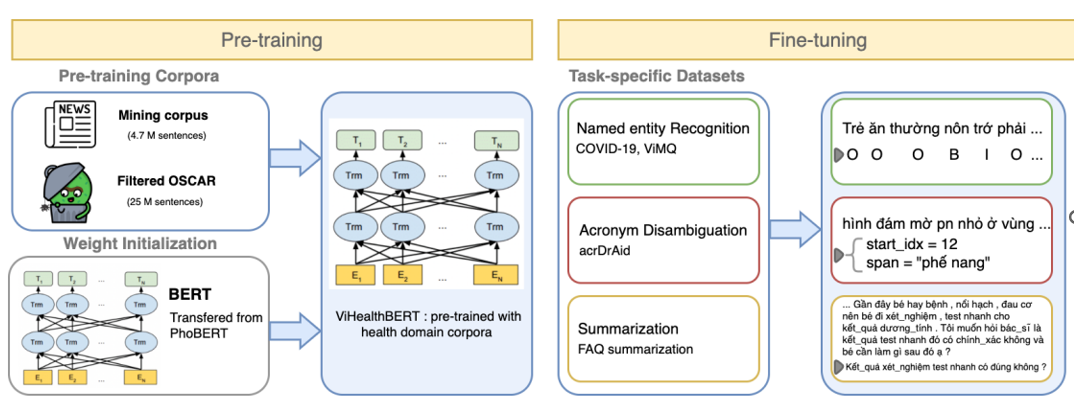
\includegraphics[scale=.75]{img/ViHealthBERT.png}
\caption{Tổng quan về quá trình pretraining và finetuning trong ViHealthBERT\cite{minh-EtAl:2022:LREC}}
\end{center}
\end{figure}

\section{Ngữ liệu huấn luyện}
\subsection{Pretraining}
ViHealthBERT sử dụng các bộ ngữ liệu \textit{Text Mining Corpus} và \textit{OSCAR} cho quá trình pretraining. Vì sử dụng trọng số huấn luyện của PhoBERT nên các bộ ngữ liệu pretraining của PhoBERT cũng được đề cập trong bảng thông số các bộ ngữ liệu pretraining (bảng~\ref{tab:pretraining-stats}).

\begin{table}[H]
\centering
\begin{tabular}{|l|c|c|}
\hline
\textbf{Dataset} & \textbf{\# Sent} & \textbf{Domain} \\ \hline
Vietnamese Wikipedia & 5M & General \\ \hline
Vietnamese news & 96M & General \\ \hline
Text Mining Corpus & 4.7M & Health, Medical \\ \hline
OSCAR's selected corpus (TF) & 25M  & Health, Medical, General \\ \hline
\end{tabular}
\caption{Thông số các bộ ngữ liệu pretraining\cite{minh-EtAl:2022:LREC}}
\label{tab:pretraining-stats}
\end{table}

\subsubsection{Text Mining Corpus}
Để xây dựng bộ ngữ liệu \textit{Text Mining Corpus}, nhóm tác giả thu thập ngữ liệu từ các trang tin điện tử, các website bệnh viện, tạp chí khoa học và sách chuyên khảo về y khoa:
\begin{itemize}
\item \textbf{Các trang tin điện tử / website bệnh viện}: nhóm tác giả dùng các từ khóa liên quan đến "y học", "vắc-xin", "y sinh" hay "sức khỏe".
\item \textbf{Các tạp chí khoa học}: nhóm tác giả trích xuất phần tóm tắt (abstract) của các tạp chí Vietnamese Medical Journal, Journal of Health and Development Studies, Journal of Medicine and Pharmacy, Medical Journal of Ho Chi Minh City.
\item \textbf{Sách chuyên khảo}: nhóm tác giả dùng bản pdf sách chuyên khảo y sinh từ website \texttt{yhoctonghop.vn}, sau đó chuyển bản pdf sang phiên bản text.
\end{itemize}
Phần ngữ liệu thô được tiền xử lý (preprocess) với các bước khử nhiễu; loại bỏ email, số điện thoại, URL; loại bỏ các câu trùng lặp sử dụng thuật toán edit-distance.

\subsubsection{OSCAR's selected corpus}
Để xây dựng Bộ ngữ liệu OSCAR\cite{ortiz-suarez-etal-2020-monolingual} nhóm tác giả đã dùng các phương pháp \textbf{Term Frequency (TF)} và \textbf{Selector} vì bộ ngữ liệu OSCAR là bộ ngữ liệu cho general-domain mà ta chỉ cần trích xuất các văn bản liên quan đến chủ đề y tế cho quá trình pretraining.

\paragraph{Term Frequency (TF)}
Phương pháp Term Frequency dựa vào tần suất xuất hiện của các từ liên quan đến chủ đề y tế để xác định xem một văn bản có thuộc chủ đề y tế hay không. Các bước thực hiện bao gồm:
\begin{enumerate}
\item Dựng một từ điển với bộ ngữ liệu thu thập được.
\item Chọn 3000 từ xuất hiện trên 10000 lần liên quan tới chủ đề y tế. Thao tác có sự kiểm tra của chuyên gia để đảm bảo các từ khóa thực sự liên quan tới chủ đề y tế.
\end{enumerate}

\paragraph{Selector}
SimCSE (\textbf{Sim}ple \textbf{C}ontrastive Learning of \textbf{S}entence \textbf{E}mbeddings)\cite{simcse2021} là một phương pháp 

\subsection{Finetuning}
\subsubsection{arcDrAid}

\subsubsection{FAQ Summarization}
\section{Thực nghiệm}
\subsection{Pretraining}
ViHealthBERT được pretrain với các task Masked Language Modeling (MLM) và Next Sentence Prediction (NSP) như PhoBERT. Nhóm tác giả đặt ra giả thuyết là những từ viết hoa thường mang ngữ nghĩa đặc biệt hơn các từ viết thường;  huấn luyện khả năng nhận biết từ viết hoa có thể giúp mô hình nhận biết các thực thể tốt hơn. Do vậy, nhóm tác giả tiến hành pretrain ViHealthBERT với task Capitalized Prediction (CP). 

Nhóm tác giả cũng thử nghiệm 2 cách tokenize ngữ liệu, bao gồm syllable-level tokenize (tách từ ở mức \textit{tiếng}) và word-level tokenize (tách từ ở mức \textit{từ}). Với syllable-level tokenizer, nhóm tác giả xác định ranh giới từ bởi dấu cách; với word-level tokenizer, nhóm tác giả sử dụng công cụ RDRSegmenter\cite{NguyenNVDJ2018} để xác định ranh giới các từ.

Mô hình được huấn luyện trên GPU A100-40GB, các thông số pretraining được thể hiện trong bảng~\ref{tab:pretraining-hyperparams}.

\begin{table}
\centering
\begin{tabular}{|c|c|}
\hline
Maximum length & 256 \\ \hline
Optimizer & AdamW \\ \hline
Batch size & 64 \\ \hline
\end{tabular}
\caption{Thông số pretraining của mô hình ViHealthBERT\cite{minh-EtAl:2022:LREC}}
\label{tab:pretraining-hyperparams}
\end{table}

\subsection{Finetuning}
\subsubsection{NER}
Nhóm tác giả finetune mô hình ViHealthBERT cho tác vụ NER trên các bộ ngữ liệu khác nhau:
\begin{itemize}
\item \textbf{PhoNER\_COVID-19}: Finetune với learning rate 5e-5, batch size 32 và train trong 30 epochs. Early stopping được thiết lập sau 5 epochs, kết quả thu được là trung bình 5 lần chạy tốt nhất với initial seeds khác nhau.
\item \textbf{Vietnamese Medical Question (ViMQ)}: Finetune với learning rate 5e-5, batch size 32 và train trong 10 epochs. Early stopping được thiết lập sau 3 epochs, kết quả thu được là trung bình 3 lần chạy tốt nhất với initial seeds khác nhau.
\end{itemize}
Nhóm tác giả finetune task NER trên server GPU A100-40GB.

\subsubsection{Acronym Disambiguation}
Với task Acronym Disambiguation, nhóm tác giả finetune mô hình với learning rate 1e-5, batch size 32 và train trong 10 epochs. Nhóm tác giả finetune task Acronym Disambiguation trên server GPU A100-40GB, kết quả thu được là trung bình 3 lần chạy với inital seeds khác nhau.

\subsubsection{FAQ Summarization}
Với task FAQ Summarization, nhóm tác giả xây dựng một mô hình Transformer với ViHealthBERT đóng vai trò là Encoder, Decoder gồm 12 Transformer Decoder block. Kích thước beam size được cài đặt là 5, batch size 64, learning rate 1e-5 và train trong 10 epochs. Nhóm tác giả finetune task FAQ Summarization trên server GPU P100-16GB, kết quả thu được là trung bình trong 3 lần chạy với initial seeds khác nhau. 

\subsection{Kết quả}
\subsubsection{Độ đo}
\paragraph{Precision, Recall và F1}
Xét bài toán phân lớp với một lớp $C$ cố định. Với \textit{TP} là số lượng mẫu thuộc về lớp $C$ được gán nhãn đúng (True Positive), \textit{FP} là số lượng mẫu không thuộc lớp $C$ nhưng được gán nhãn đúng (False Positive) và \textit{FN} là số lượng mẫu thuộc lớp $C$ và được gán nhãn sai (False Negative). Công thức tính Precision, Recall và F1-Score khi đó được định nghĩa như sau:
\begin{equation}
\begin{aligned}
Precision~(P) &= \frac{TP}{TP + FP} \\
Recall~(R) &= \frac{TP}{TP + FN} \\
F1 &= \frac{2PR}{P + R}
\end{aligned}
\end{equation}

\paragraph{Macro, Micro} Lấy ví dụ với Macro Precision và Micro Precision trong bài toán phân lớp với $n$ lớp. Với $TP_1, TP_2, .., TP_n$ là số lượng mẫu True Positive và $FP_1, FP_2, .., FP_n$ là số lượng mẫu False Positive của $n$ lớp. Khi đó độ đo Micro Precision được tính toán với số lượng mẫu $TP$ và $FP$ của từng lớp, trong khi độ đo Macro Precision là trung bình cộng Precision của các lớp:

\begin{equation}
\begin{aligned}
Precision_{micro} &= \frac{TP_1 + TP_2 + .. + TP_n}{(TP_1 + FP_1) + (TP_2 + FP_2) + .. + (TP_n + FP_n)} = \frac{\displaystyle\sum_{i = 1}^n TP_i}{\displaystyle\sum_{i = 1}^n (TP_i + FP_i)} \\
Precision_{macro} &= \frac{1}{n}\left[\left(\frac{TP_1}{TP_1 + FP_1}\right) + \left(\frac{TP_2}{TP_2 + FP_2}\right) + .. + \left(\frac{TP_n}{TP_n + FP_n}\right)\right] = \frac{1}{n}\sum_{i = 1}^n \frac{TP_i}{TP_i + FP_i}
\end{aligned}
\end{equation}
Các độ đo Micro/Macro Recall, F1 có cách tính tương tự.

\paragraph{ROUGE}
\textbf{R}ecall-\textbf{O}riented \textbf{U}nderstudy for \textbf{G}isting \textbf{E}valuation\cite{lin-2004-rouge} là độ đo được thiết kế cho task Text Summarization. Với $n$ là chiều dài của $n$-grams và $gram_n$, $Count_{match}(gram_n)$ là số lượng $n$-grams nhiều nhất xuất hiện trong bản tóm tắt do máy đưa ra và bản tóm tắt của chuyên gia. Độ đo ROUGE-$N$ khi đó được định nghĩa như sau:
\begin{equation}
\text{ROUGE-}N = \frac{\displaystyle\sum_{S \in {ReferenceSummaries}}\left(\sum_{gram_n \in S}Count_{match}(gram_n)\right)}{\displaystyle\sum_{S \in {ReferenceSummaries}}\left(\sum_{gram_n \in S}Count(gram_n)\right)}
\end{equation}
Các độ đo ROUGE-$N$ phổ biến bao gồm ROUGE-1 (dựa trên các \textit{unigrams}) và ROUGE-2 (dựa trên các \textit{bigrams}). 

Ngoài ROUGE-$N$, độ đo ROUGE-$L$ dựa trên \textit{dãy con chung dài nhất (Longest Common Subsequence - LCS)} cũng được sử dụng làm độ đo cho các task Text Summarization. Gọi $X$ và $Y$ lần lượt là 2 bản tóm tắt do máy và do chuyên gia thực hiện, $m$ và $n$ lần lượt là độ dài của $X$ và $Y$. Khi đó độ đo ROUGE-$L$ được tính như sau:

\begin{equation}
\begin{aligned}
R_{lcs} &= \frac{LCS(X, Y)}{m} \\
P_{lcs} &= \frac{LCS(X, Y)}{n} \\
F_{lcs} &= \frac{(1 + \beta^2)R_{lcs}P_{lcs}}{R_{lcs} + \beta^2P_{lcs}}
\end{aligned}
\end{equation}
$LCS(X, Y)$ trong công thức được định nghĩa là dãy con chung dài nhất của $X$ và $Y$, $\displaystyle \beta = \frac{P_{lcs}}{R_{lcs}}$. Khi đó, độ đo ROUGE-$L$ giữa 2 văn bản $X$ và $Y$ bằng $F_{lcs}$ trong công thức bên trên.

\subsubsection{NER}
Nhóm tác giả sử dụng độ đo Micro F1 và Macro F1 cho task NER. Kết quả thực nghiệm của nhóm tác giả được thể hiện trong bảng~\ref{tab:experiments-ner}. Nhìn chung, mô hình ViHealthBERT cho ra kết quả tốt hơn PhoBERT với tất cả các thông số huấn luyện khác nhau. Cụ thể:
\begin{itemize}
\item Với bộ ngữ liệu PhoNER\_COVID-19, kết quả tốt nhất của ViHealthBERT đạt 96.77\% Macro-F1 (hơn PhoBERT 2.2\%) và 96.77\% Micro-F1 (hơn PhoBERT 4.7\%).
\item Với bộ ngữ liệu ViMQ, kết quả tốt nhất của ViHealthBERT đạt 86.98\% Macro-F1 (hơn PhoBERT 2.26\%) và 86.21\% (hơn PhoBERT 3.97\%).
\end{itemize}

\begin{table}
\centering
\resizebox{\textwidth}{!}{
\begin{tabular}{| *{8}{l|} }
\hline
Model & Tokenize-level & Pre-training data & Pre-training task & \multicolumn{2}{c|}{COVID-19} & \multicolumn{2}{c|}{ViMQ} \\
& & & & Mac-F1 & Mic-F1 & Mac-F1 & Mic-F1 \\ \hline
PhoBERT\textsubscript{base} & word & * & MLM & 0.942 & 0.920 & 0.8470 & 0.8224 \\ 
PhoBERT\textsubscript{large} & word & * & MLM & 0.945 & 0.931 & 0.8524 & 0.8257 \\ \hline
ViHealthBERT & word & * + our & MLM & \textbf{0.9677} & \textbf{0.9677} & 0.8601 & 0.8432 \\ 
ViHealthBERT & word & * + our & MLM + NSP & 0.9674 & 0.9674 & 0.8562 & 0.8441 \\
ViHealthBERT & word & * + our & MLM + CP & 0.9677 & 0.9677 & 0.8678 & 0.8397 \\
ViHealthBERT & word & * + our & MLM + NSP + CP & 0.9662 & 0.9619 & 0.8526 & 0.8383 \\ \hline
ViHealthBERT & syllable & * + our & MLM & 0.9652 & 0.9653 & 0.8575 & 0.8481 \\
ViHealthBERT & syllable & * + our & MLM + NSP & 0.9673 & 0.9673 & 0.8610 & 0.8440 \\
ViHealthBERT & syllable & * + our & MLM + CP & 0.9672 & 0.9677 & 0.8664 & 0.8567 \\
ViHealthBERT & syllable & * + our & MLM + NSP + CP & 0.9665 & 0.9664 & 0.8676 & 0.8641 \\ \hline
ViHealthBERT & syllable & * + our + TF & MLM & 0.9639 & 0.9641 & \textbf{0.8698} & \textbf{0.8621} \\
ViHealthBERT & syllable & * + our + TF & MLM + CP & 0.9629 & 0.9629 & 0.8632 & 0.8501 \\ \hline
\end{tabular}}
\caption{Kết quả thực nghiệm của nhóm tác giả với task NER\cite{minh-EtAl:2022:LREC}. * là bộ ngữ liệu huấn luyện của PhoBERT, \textit{our} và \textit{TF} là các bộ ngữ liệu huấn luyện đã nêu trong phần Ngữ liệu huấn luyện.}
\label{tab:experiments-ner}
\end{table}

\subsubsection{Acronym Disambiguation}
Nhóm tác giả sử dụng độ đo Macro Precision, Macro Recall và Macro F1 cho task Acronym Disambiguation. Kết quả thực nghiệm của nhóm tác giả được trình bày ở bảng~\ref{tab:experiments-ad}. Mô hình ViHealthBERT cho kết quả tốt hơn PhoBERT, cụ thể:
\begin{itemize}
\item Các kết quả tốt nhất của ViHealthBERT tăng 1.17\% Macro Precision, 6.28\% Macro Recall và 4.19\% Macro F1 so với PhoBERT\textsubscript{base}.
\item Các kết quả tốt nhất của ViHealthBERT tăng 1.64\% Macro Precision, 10.71\% Macro Recall và 7.14\% Macro F1 so với PhoBERT\textsubscript{large}.
\end{itemize}

\begin{table}
\centering
\resizebox{\textwidth}{!}{
\begin{tabular}{| *{7}{l|} }
\hline
Model & Tokenize-level & Pre-training data & Pre-training task & Mac-Pre & Mac-Rec & Mac-F1 \\ \hline
PhoBERT\textsubscript{base} & word & * & MLM & 0.9197 & 0.7481 & 0.8251 \\ 
PhoBERT\textsubscript{large} & word & * & MLM & 0.9150 & 0.7038 & 0.7956 \\ \hline
ViHealthBERT & word & * + our & MLM & 0.9281 & 0.7565 & 0.8336 \\ 
ViHealthBERT & word & * + our & MLM + NSP & 0.9320 & 0.7562 & 0.8349 \\
ViHealthBERT & word & * + our & MLM + CP & 0.9235 & 0.7605 & 0.8341 \\
ViHealthBERT & word & * + our & MLM + NSP + CP & 0.9212 & 0.7583 & 0.8318 \\ \hline
ViHealthBERT & syllable & * + our & MLM & 0.9652 & 0.7928 & 0.8555 \\
ViHealthBERT & syllable & * + our & MLM + NSP & 0.9314 & \textbf{0.8109} & \textbf{0.8670} \\
ViHealthBERT & syllable & * + our & MLM + CP & \textbf{0.9402} & 0.7838 & 0.8559 \\
ViHealthBERT & syllable & * + our & MLM + NSP + CP & 0.9362 & 0.777 & 0.8493 \\ \hline
ViHealthBERT & syllable & * + our + TF & MLM & 0.9315 & 0.7878 & 0.8537 \\
ViHealthBERT & syllable & * + our + TF & MLM + CP & 0.9287 & 0.7927 & 0.8553 \\ \hline
\end{tabular}}
\caption{Kết quả thực nghiệm của nhóm tác giả với task Acronym Disambiguation\cite{minh-EtAl:2022:LREC}. * là bộ ngữ liệu huấn luyện của PhoBERT, \textit{our} và \textit{TF} là các bộ ngữ liệu huấn luyện đã nêu trong phần Ngữ liệu huấn luyện.}
\label{tab:experiments-ad}
\end{table}

\subsubsection{FAQ Summarization}
Nhóm tác giả sử dụng độ đo ROUGE-1, ROUGE-2 và ROUGE-$L$ cho task FAQ Summarization. Kết quả thực nghiệm của nhóm tác giả được trình bày ở bảng~\ref{tab:experiments-faq}. Mô hình ViHealthBERT đạt hiệu quả cao hơn PhoBERT, cụ thể tăng 3.3\% ROUGE-1, 3.17\% ROUGE-2 và 2.66\% ROUGE-$L$. 

\begin{table}
\centering
\resizebox{\textwidth}{!}{
\begin{tabular}{| *{7}{l|} }
\hline
Model & Tokenize-level & Pre-training data & Pre-training task & R-1 & R-2 & R-L \\ \hline
PhoBERT\textsubscript{base} & word & * & MLM & 47.15 & 28.18 & 41.16 \\ \hline
ViHealthBERT & word & * + our & MLM & \textbf{50.45} & \textbf{31.35} & \textbf{43.85} \\ 
ViHealthBERT & word & * + our & MLM + NSP & 49.06 & 29.7 & 42.56 \\
ViHealthBERT & word & * + our & MLM + CP & 47.85 & 29.81 & 42.04 \\
ViHealthBERT & word & * + our & MLM + NSP + CP & 50.4 & 31.15 & 43.78 \\ \hline
ViHealthBERT & syllable & * + our & MLM & 48.47 & 28.65 & 41.77 \\
ViHealthBERT & syllable & * + our & MLM + NSP & 49.92 & 30.77 & 43.37 \\
ViHealthBERT & syllable & * + our & MLM + CP & 48.56 & 29.20 & 41.96 \\
ViHealthBERT & syllable & * + our & MLM + NSP + CP & 48.33 & 30.35 & 42.36 \\ \hline
ViHealthBERT & syllable & * + our + TF & MLM & 48.32 & 29.17 & 42.07 \\
ViHealthBERT & syllable & * + our + TF & MLM + CP & 49.45 & 30.86 & 43.26 \\ \hline
\end{tabular}}
\caption{Kết quả thực nghiệm của nhóm tác giả với task FAQ Summarization\cite{minh-EtAl:2022:LREC}. * là bộ ngữ liệu huấn luyện của PhoBERT, \textit{our} và \textit{TF} là các bộ ngữ liệu huấn luyện đã nêu trong phần Ngữ liệu huấn luyện.}
\label{tab:experiments-faq}
\end{table}

\subsection{Thực nghiệm của nhóm}
Nhóm tiến hành finetune lại mô hình ViHealthBERT được công bố trên GitHub\footnote{\href{https://github.com/demdecuong/vihealthbert}{https://github.com/demdecuong/vihealthbert}} và Huggingface\footnote{\href{https://huggingface.co/demdecuong/vihealthbert-base-word}{https://huggingface.co/demdecuong/vihealthbert-base-word}} cho 2 tasks NER và Acronym Disambiguation.

\subsubsection{NER}
Với task NER, nhóm sử dụng bộ ngữ liệu PhoNER\_COVID-19. Các bước finetune được thực hiện như nhóm tác giả đã đề cập trong bài báo với các thông số huấn luyện được trình bày trong bảng~\ref{tab:experiments-self-ner}. Kết quả huấn luyện được trình bày trong bảng~\ref{tab:expreiments-self-ner-results}, chi tiết ở notebook \texttt{ViHealthBERT\_NER.ipynb}.

\begin{table}
\centering
\begin{tabular}{|c|c|}
\hline
Epochs & 10 \\ \hline
Batch size & 16 \\ \hline
Max seq. length & 70 \\ \hline
Learning rate & 5e-5 \\ \hline
Dropout rate & 0.1 \\ \hline
\end{tabular}
\caption{Thông số huấn luyện task NER của nhóm.}
\label{tab:experiments-self-ner}
\end{table}

\begin{table}
\centering
\begin{tabular}{|l|l|l|l|}
\hline
\textbf{label}        & \textbf{precision} & \textbf{recall} & \textbf{f1-score} \\ \hline
DATE                  & 0.9909             & 0.9921          & 0.9915            \\ \hdashline
SYMPTOM\_AND\_DISEASE & 0.9322             & 0.9040          & 0.9179            \\ \hdashline
NAME                  & 0.9073             & 0.9073          & 0.9073            \\ \hdashline
LOCATION              & 0.9529             & 0.9381          & 0.9454            \\ \hdashline
PATIENT\_ID           & 0.9857             & 0.9841          & 0.9849            \\ \hdashline
TRANSPORTATION        & 0.9442             & 0.9637          & 0.9538            \\ \hdashline
GENDER                & 1.0000             & 0.9776          & 0.9887            \\ \hdashline
ORGANIZATION          & 0.9064             & 0.9182          & 0.9123            \\ \hdashline
JOB                   & 0.8659             & 0.8208          & 0.8427            \\ \hdashline
AGE                   & 0.9803             & 0.9681          & 0.9741            \\ \hline
\textbf{micro avg}    & 0.9592             & 0.9497          & 0.9545            \\ \hline
\textbf{macro avg}    & 0.9592             & 0.9497          & 0.9544            \\ \hline
\end{tabular}
\caption{Kết quả finetune mô hình ViHealthBERT cho tác vụ NER trên tập test của bộ ngữ liệu PhoNER\_COVID-19}
\label{tab:expreiments-self-ner-results}
\end{table}
Với mô hình đã được finetune, nhóm tiến hành xây dựng một ứng dụng hỗ trợ trích xuất triệu chứng từ miêu tả của bệnh nhân. Đây là đồ án thực hành của nhóm, sẽ được trình bày chi tiết trong phần Báo cáo đồ án.

\subsubsection{Acronym Disambiguation}
Với task Acronym Disambiguation, nhóm thực hiện lại các bước finetune mô hình ViHealthBERT như trong bài báo đã đề cập, các thông số huấn luyện được trình bày trong bảng~\ref{tab:experiments-self-ad}.

\begin{table}
\centering
\begin{tabular}{|c|c|}
\hline
Epochs & 100 \\ \hline
Batch size & 16 \\ \hline
Max seq. length & 256 \\ \hline
Adam epsilon & 1e-9 \\ \hline
Learning rate & 1e-5 \\ \hline
Dropout rate & 0.1 \\ \hline
\end{tabular}
\caption{Thông số huấn luyện task Acronym Disambiguation của nhóm.}
\label{tab:experiments-self-ad}
\end{table}

Kết quả huấn luyện đạt độ chính xác (Accuracy) là 0.8599 trên tập test của bộ ngữ liệu arcDrAid. Một ví dụ cho task Acronym Disambiguation với mô hình nhóm đã finetune được thể hiện trong hình~\ref{fig:demo-wsd-output}. Chi tiết ở notebook \texttt{ViHealthBERT\_WSD.ipynb} (huấn luyện) và \texttt{demo\_predict\_wsd.ipynb} (demo).

\begin{figure}
\centering
\resizebox{\textwidth}{!}{
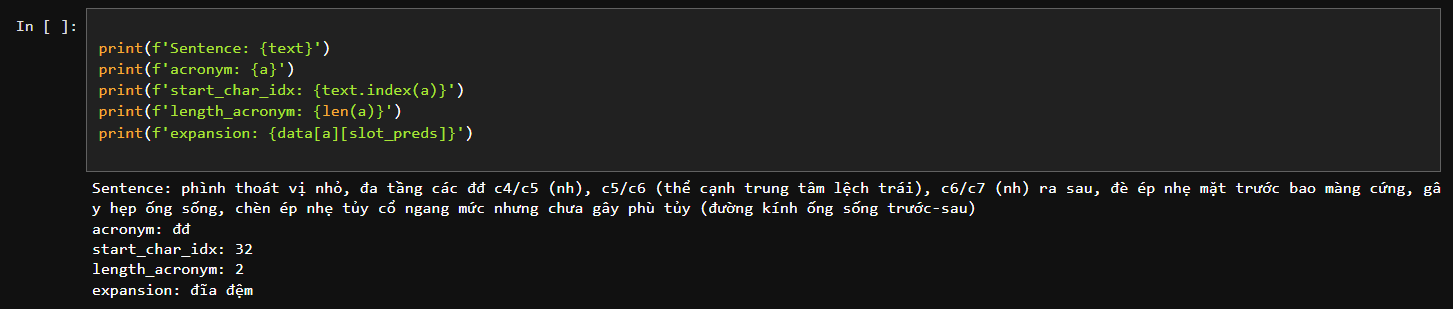
\includegraphics{img/wsd-demo.PNG}
}
\caption{Ví dụ cho task Acronym Disambiguation với mô hình nhóm đã finetune}
\label{fig:demo-wsd-output}
\end{figure}
\section{Tổng kết}
Qua đồ án này, nhóm xin tổng kết lại các nội dung đã thực hiện:
\begin{itemize}
\item Nhóm finetune mô hình ViHealthBERT cho tác vụ NER dùng bộ ngữ liệu  PhoNER\_COVID-19. Mô hình sau khi finetune đạt được 95\% Precision, 94\% Recall và 95\% F1-Score khi đối chiếu với tập test của bộ ngữ liệu PhoNER\_COVID-19.

\item Từ mô hình đã huấn luyện, nhóm xây dựng một ứng dụng hỗ trợ trích xuất các triệu chứng bệnh từ mô tả của người dùng.
\end{itemize}
Trong tương lai, nhóm đề xuất một số hướng cải tiến ứng dụng nhằm mang lại hiệu quả và trải nghiệm tốt nhất cho người sử dụng. Một số hướng cải tiến nhóm đề xuất bao gồm:
\begin{itemize}
\item Hỗ trợ nhập liệu từ file. Khi đó hệ thống có thể trích xuất và đưa ra danh sách triệu chứng của nhiều bệnh nhân cùng lúc.

\item Xây dựng một module chẩn đoán bệnh dựa trên danh sách các triệu chứng. Danh sách triệu chứng hiện có sẽ được đưa qua một mạng neural đơn giản để đưa ra chẩn đoán nhanh. Tuy nhiên người bệnh vẫn cần tham khảo ý kiến của bác sĩ để có được chẩn đoán chính xác nhất.
\end{itemize}

% \cleardoublepage
\phantomsection
\addcontentsline{toc}{section}{Tài liệu}
\bibliographystyle{acm}
\bibliography{citation/ref}
\end{document}